\documentclass{beamer}
 
\usepackage[utf8]{inputenc}
\usepackage{braket}
\usepackage{mathtools} % Needed for \prescript
\usetheme{Boadilla}
\setbeamertemplate{navigation symbols}{}
\usepackage{subfig}
\usepackage{hyperref}

\captionsetup[subfigure]{labelformat=empty}
\captionsetup[figure]{labelformat=empty}

\newcommand{\tot}{\mathrm{tot}}
\DeclareMathOperator{\Tr}{Tr}

%Information to be included in the title page:
\title{LSTM Tagger}
\author{Philipp Windischhofer}
%\institute{ETH Zürich}
\date{\today}
  
\begin{document}
 
\frame{\titlepage}

%\begin{frame}
%\frametitle{Table of Contents}
%\tableofcontents
%\end{frame}

\begin{frame}
  \frametitle{The Setup}

  \begin{block}{Goal}
    Train a binary neural-network based classifier that can distinguish between $b$- and non-$b$-jets, using the raw jet data as input.
  \end{block}

  \begin{itemize}
  \item use \textsl{tracks} as the primary source of information
  \item number of tracks is unknown a-priori $\rightarrow$ cannot use an architecture that expects a fixed number of inputs
  \item currently looking into recurrent neural networks / LSTM networks
  \end{itemize}
\end{frame}

\begin{frame}
  \frametitle{The Workflow}
  \framesubtitle{Training}
  \begin{itemize}
  \item match tracks to their associated jets (contained in different ROOT trees)
    \begin{itemize}
      \item done \textsl{ahead} of training
    \end{itemize}
  \item save matched tracks / jets to disk (HDF5)
  \item for each track in the jet, feed the track parameters into the classifier network during training
    \begin{itemize}
      \item (may) use $p_T$ ordering, i.e.~hardest track first
    \end{itemize}
  \item supervised training: provide a binary (0/1) output value for each jet (from MC truth)
  \end{itemize}

\end{frame}

\begin{frame}
  \frametitle{Results so far (work in progress)}
  trained a number of LSTM networks, scanned the hyperparameters:
    \begin{itemize}
    \item number of nodes in each layer
    \item number of layers
    \item number of training epochs
    \end{itemize}
  
  Details of the training:
  \begin{itemize}
  \item training dataset contains 100-150k jets
  \item training/validation split 80:20
  \item batch size: 1k jets (also tried unbatched training)
  \end{itemize}

  Progress w.r.t. last time:
  \begin{itemize}
    \item made code (much) more flexible
    \item ready to efficiently ramp up training \& try different network types
  \end{itemize}  
\end{frame}

\begin{frame}
  \frametitle{different network shapes (unbatched)}
  \begin{itemize}
  \item batch size = 1
    \item labelling: \textsl{number nodes / number layers}
  \end{itemize}
  
    \begin{figure}[htb]
    \centering
    \subfloat[][]{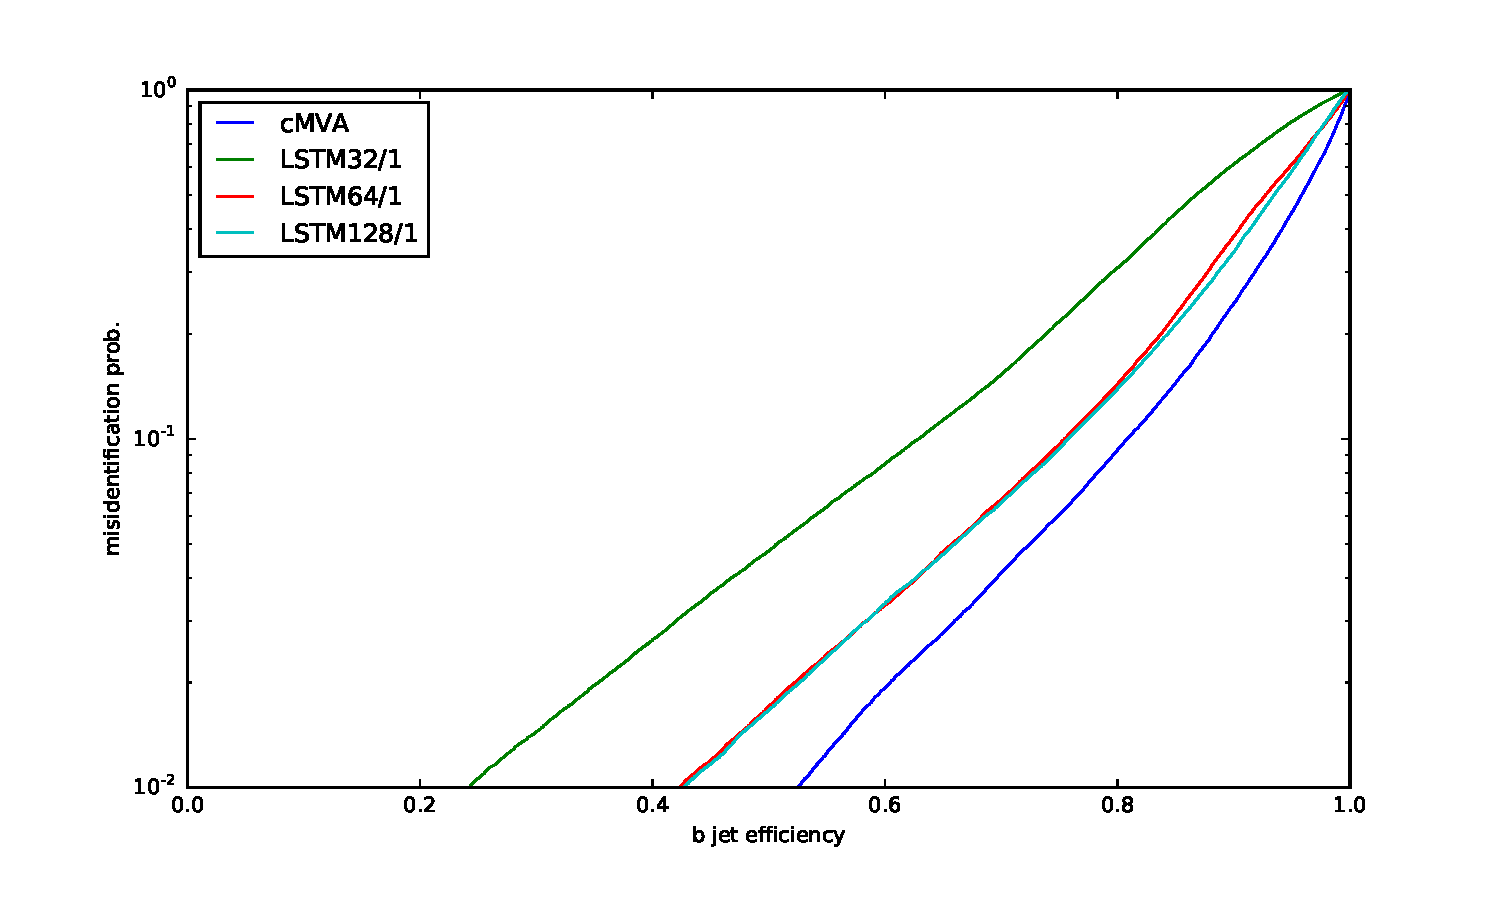
\includegraphics[width =0.9\textwidth]{./1layers.pdf}}	
  \end{figure}

\end{frame}

\begin{frame}
  \frametitle{using less information}
    \begin{figure}[htb]
    \centering
    \subfloat[][]{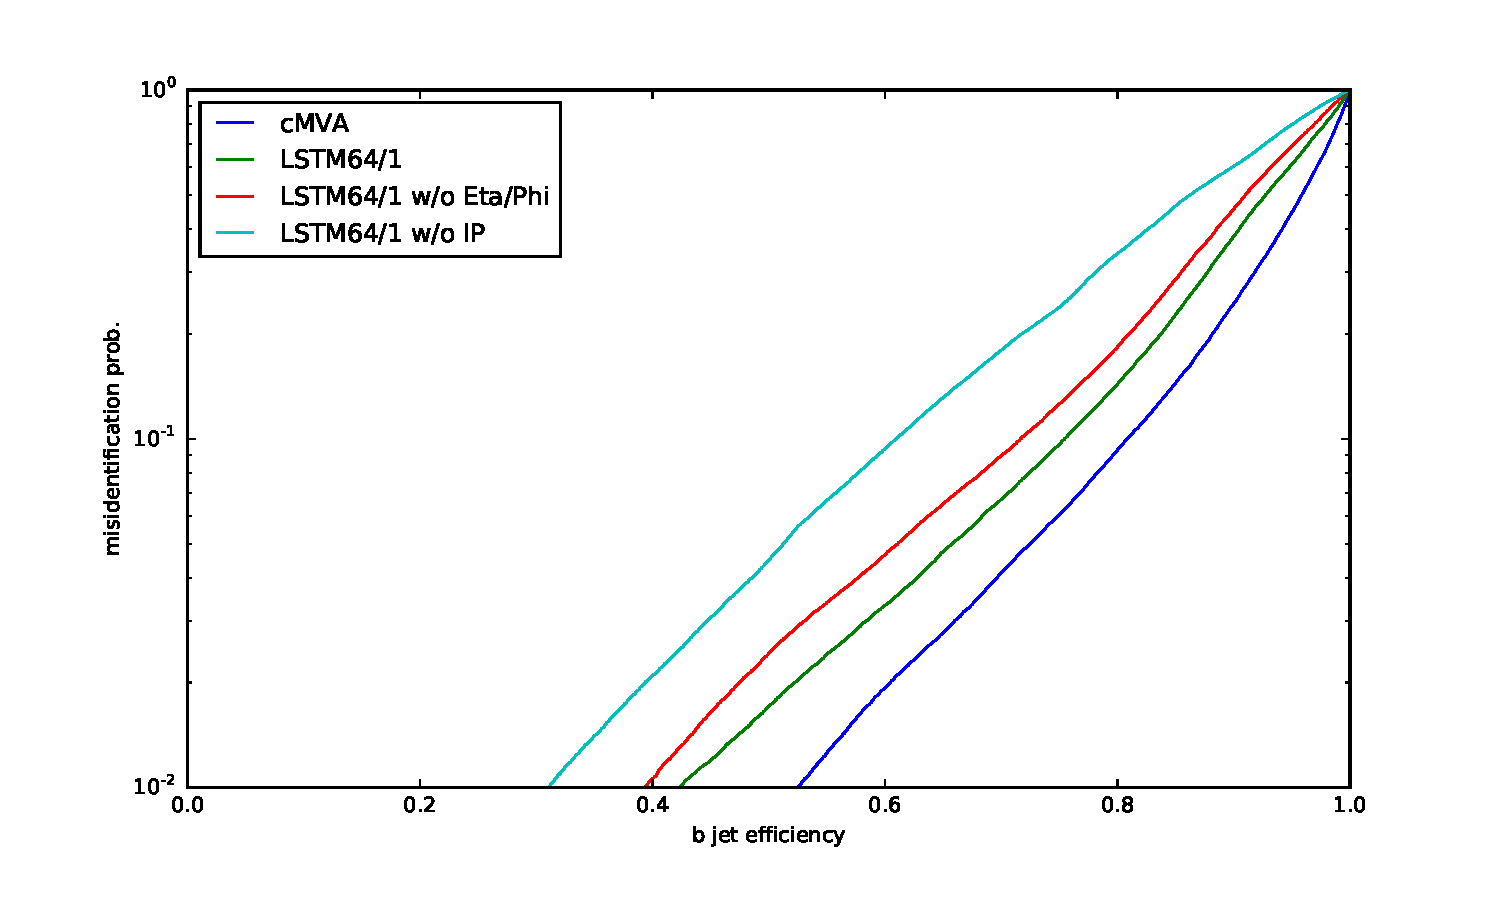
\includegraphics[width =0.9\textwidth]{./removed_parameters.pdf}}	
  \end{figure}

\end{frame}

\begin{frame}
  \frametitle{batched training}
  batch size = 1k jets

    \begin{figure}[htb]
    \centering
    \subfloat[][]{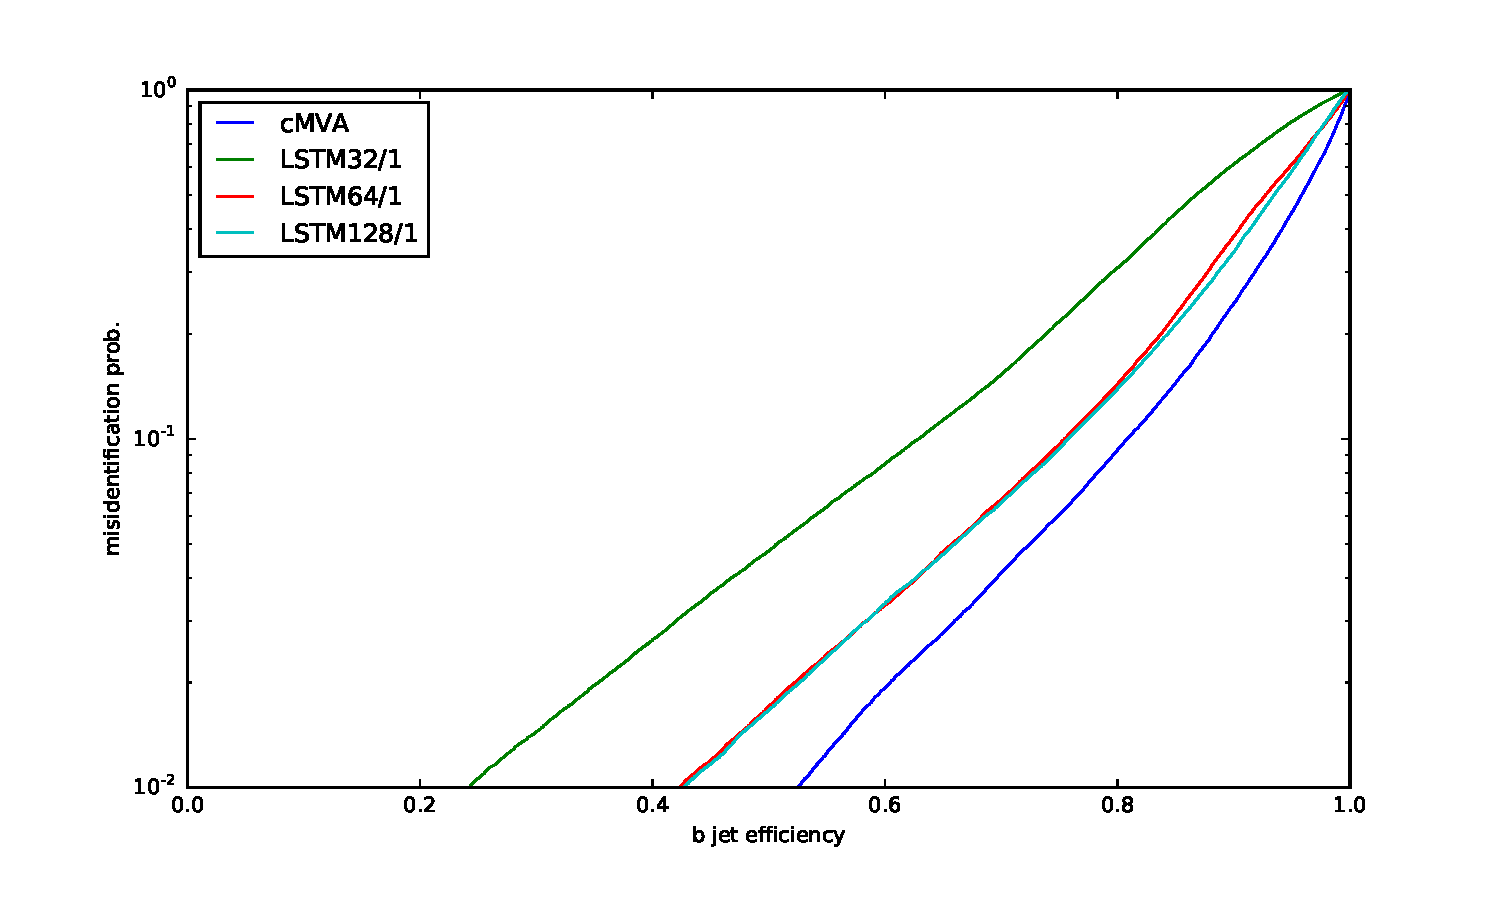
\includegraphics[width =1.0\textwidth]{./1layers.pdf}}	
  \end{figure}

\end{frame}

\begin{frame}
  \frametitle{Conclusions}

\end{frame}

\end{document}
